% Generated by build_report.py; shared presentation content.
\section{Kiến trúc mô hình BR-Dummy: Geo-I, mạng đường và các cơ chế}
Đọc theo số \textbf{1 $\to$ 2 $\to$ 3a/3b $\to$ 4 $\to$ server $\to$ 5}. Khung xanh là mô hình; A/B là hai cơ chế Boundary tùy chọn.

\begin{center}
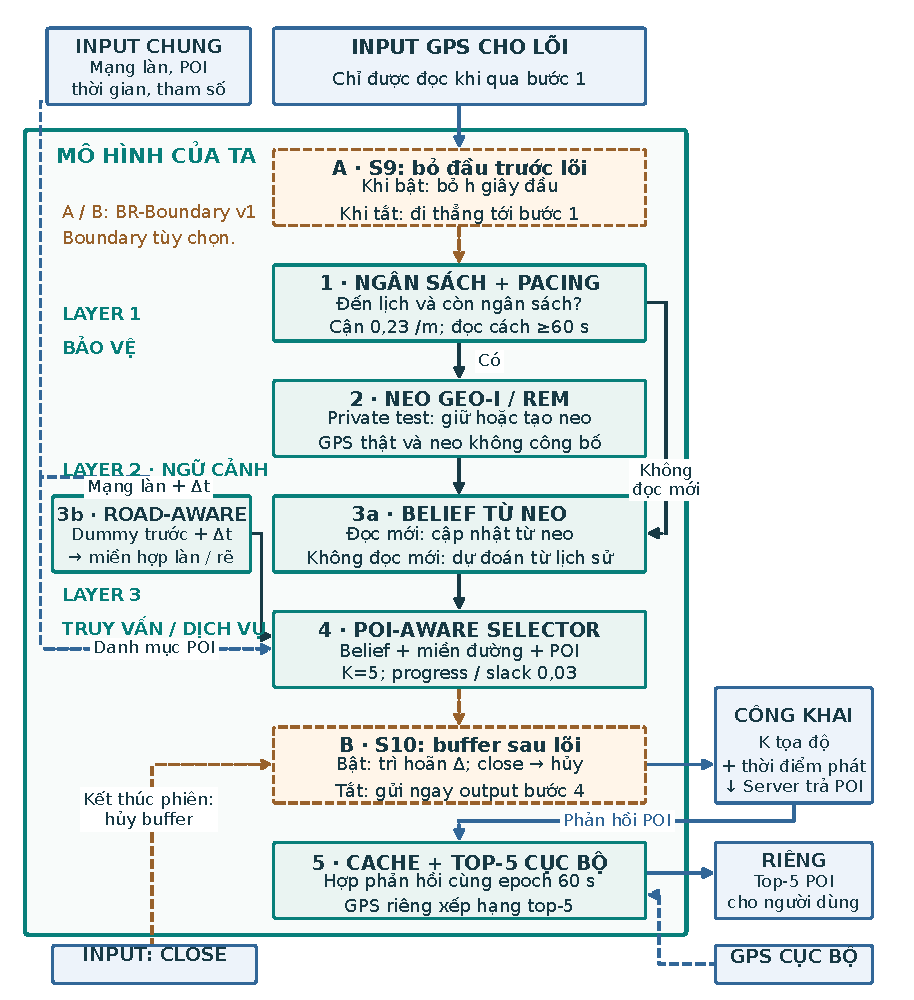
\includegraphics[width=\linewidth,height=0.79\textheight,keepaspectratio]{figures/architecture_report_flow.pdf}
\end{center}
Bước 1 không cho đọc GPS mới thì bỏ qua bước 2. Belief và road-aware cùng đưa đầu vào cho bộ chọn. Cache nhận phản hồi từ server. GPS thật chỉ xếp hạng cục bộ sau khi tạo query.


\clearpage
\subsection{Vai trò các khối và hai cấu hình Geo-I}
\begingroup\small
\begin{longtable}{@{}P{5.006cm}P{11.913cm}@{}}
\toprule
\textbf{Component} & \textbf{Vai trò trọng tâm}\\\midrule
\endfirsthead
\toprule
\textbf{Component} & \textbf{Vai trò trọng tâm}\\\midrule
\endhead
\bottomrule\endfoot
1. Ngân sách + pacing — S2/S3 & Giới hạn việc đọc GPS trong phiên; giữa các lần đọc chỉ xử lý trạng thái đã bảo vệ.\\
\addlinespace[3pt]
2. Neo Geo-I / REM — S1/S2 & Private test giữ hoặc tạo neo riêng tư; tái dùng giảm mẫu nhiễu mới khi quan sát lặp.\\
\addlinespace[3pt]
3a. Belief từ neo — dịch vụ & Ước lượng vùng vị trí từ lịch sử neo; không coi một neo nhiễu là vị trí chính xác.\\
\addlinespace[3pt]
3b. Road-aware — S3 & Tạo miền dummy tới được theo làn, luật rẽ và thời gian từ dummy bước trước.\\
\addlinespace[3pt]
4. POI-aware selector — dịch vụ & Chọn K query phủ POI bổ sung nhau; progress/slack giúp di chuyển tới vùng phục vụ tốt hơn.\\
\addlinespace[3pt]
5. Cache + top-5 cục bộ — dịch vụ & Hợp phản hồi còn hiệu lực trong epoch; dùng GPS tại thiết bị để xếp hạng top-5.\\
\addlinespace[3pt]
A. Boundary đầu — S9 & Bỏ h giây đầu trước lõi để GPS đoạn này không đi vào trạng thái neo.\\
\addlinespace[3pt]
B. Boundary cuối — S10 & Buffer output sau lõi; khi kết thúc, hủy phần chưa phát thay vì flush.\\
\end{longtable}
\endgroup
Bộ chọn dummy chỉ dùng neo đã bảo vệ và dữ liệu công khai. K dummy không tự tạo k-anonymity. Boundary đã kiểm tra tích hợp, chưa benchmark kết hợp với dịch vụ.

\subsection{Định lượng hai cấu hình Geo-I}
\textbf{GeoI-Paced:} cấu hình đối chứng nội bộ. \textbf{GeoI-Slack:} bản hiện tại, thêm độ linh hoạt khi chọn dummy. Hai bản cùng ngân sách riêng tư và cùng dịch vụ.

\begingroup\small
\begin{longtable}{@{}P{3.938cm}P{6.350cm}P{6.350cm}@{}}
\toprule
\textbf{Tham số / component} & \textbf{GeoI-Paced} & \textbf{GeoI-Slack}\\\midrule
\endfirsthead
\toprule
\textbf{Tham số / component} & \textbf{GeoI-Paced} & \textbf{GeoI-Slack}\\\midrule
\endhead
\bottomrule\endfoot
Neo / ngân sách & $\varepsilon$\_\allowbreak{}test = $\varepsilon$\_\allowbreak{}release = 0,01 /m; θ = 200 m; cận phiên 0,23 /m & Giống GeoI-Paced\\
\addlinespace[3pt]
Đọc GPS / cache & Đọc cách $\ge$60 giây; cache cùng epoch 60 giây & Giống GeoI-Paced\\
\addlinespace[3pt]
Dịch vụ & K=5 điểm; L=10 POI/loại/điểm; chọn top-5 tại thiết bị & Giống GeoI-Paced\\
\addlinespace[3pt]
Slack & Không nới điểm mục tiêu của bộ chọn & Cho phép giảm tối đa 0,03 điểm mục tiêu để di chuyển hữu ích hơn; không phải giảm Recall 3\%\\
\end{longtable}
\endgroup
\key{Đóng góp: phối hợp lịch sử Geo-I đã bảo vệ, ngân sách, mạng làn và mục tiêu phủ POI. Geo-I + dummy đã có tiền lệ [\href{https://wrap.warwick.ac.uk/id/eprint/183198/1/WRAP-privacy-preserving-querying-mechanism-high-utility-electric-vehicles-2024.pdf}{R12}]; lợi ích của cách phối hợp phải được kiểm tra bằng benchmark.}

